\chapter{The Deep Nature of Quantum Mechanics}
\label{chap:qm-as-compression}

\section{Introduction: The Ubiquitous Wave}

What is the deep, foundational nature of Quantum Mechanics and its mysterious wavefunction? 

At its core, the microscopic building blocks of our universe are astonishingly simple—a small, elegant set of quantum fields characterized by just a handful of fundamental parameters, yet capable of producing an enormous expanse of emergent richness.

The complex-valued amplitudes in the wavefunction do all the heavy lifting.
Crucial phenomena such as interference, entanglement, quantum tunneling, and superpositions are not separate arbitrary features; they are the mathematical consequences of reality existing within a complex-valued Hilbert space. 

If we temporarily step back from these specific technical features, a deeper, more primitive question remains: \emph{Why does everything at the subatomic level appear to behave like a wave in the first place?}

\subsection*{The Movie Analogy}

Consider a conventional MPEG-compressed digital movie.
Each individual frame is fundamentally composed of discrete, static pixels.
If we were conscious observers made of pixels living entirely inside such a digital movie, what would we perceive as our "laws of physics"?

We would observe that our constituent pixels follow mysterious, abstract, yet completely deterministic wave-like patterns across time.
To a pixel-physicist, these transitions would look like fundamental laws.
In reality, these patterns are merely the mathematical output of the Discrete Cosine Transform (DCT) or Fourier transforms—the underlying mathematical tools that MPEG codecs use to compress raw pixel grids into a maximally dense format for efficient transmission and storage.

From this informational perspective, the Quantum Mechanical wavefunction is simply an advanced, complex-valued version of the sinusoidal building blocks used in JPEG or MPEG algorithms.
Just as a spatial Fourier transform spreads concentrated image information across a spectrum of frequency coefficients, the wavefunction distributes probability amplitudes across basis states in Hilbert space.

Waves—and complex-valued amplitudes in particular—are exceptionally efficient at densely encoding relational information.
They produce exactly the kind of spatial smoothness, structural continuity, and predictive regularity that intelligent observers require to exist and reason.

\section{The Dithering Analogy}

The evolution of the wavefunction itself is entirely deterministic; randomness emerges only when a macroscopic observer attempts to interpret this smooth, continuous wave in terms of discrete, localized particles. 

Consider a 3D graphics engine rendering a perfectly smooth, analytically defined sphere with an intended shading intensity of exactly $0.85$.
If the underlying display hardware is strictly limited to discrete integer outputs of either $0.8$ or $0.9$, it lacks the structural resolution to render the true value directly.
To compensate, the software employs \textbf{dithering}—a probabilistic rendering rule that distributes discrete values across adjacent pixels such that the average intensity across the surface mathematically approximates the ideal fractional value, smoothing out jagged banding and moiré patterns.

In this light, a quantum superposition state:
\[
|\psi\rangle = \alpha |0.8\rangle + \beta |0.9\rangle
\]
can be viewed as nature’s highly advanced, complex-valued implementation of this exact computational optimization. 

Just as digital dithering maximizes perceived visual quality while minimizing hardware memory consumption, the Born Rule allows the universe to maintain a high-fidelity, compressed informational state within a physical framework operating under strictly limited observables.
Quantum mechanics may simply be the most efficient rendering engine mathematically possible—using complex-valued probability amplitudes to maximize the fidelity of the universe with a minimal expenditure of underlying data.

\section{From Kolmogorov to Spectral Complexity}

Kolmogorov complexity provides a theoretical foundation for minimal description lengths.
However, because it relies on the binary halting state of a Turing machine, it is fundamentally discrete, discontinuous, and uncomputable.
It is difficult to see how such a jagged, "jumpy" informational measure could smoothly support stable prediction, continuous spacetime geometry, or the gradual evolutionary reasoning of an intelligent observer.

More importantly, observational evidence suggests that physical systems already possess a natural, inherent mode of information representation: their decomposition into \textbf{spectral modes}.
This motivates us to replace abstract algorithmic complexity with a physically grounded, continuous alternative:

\begin{definition}{Spectral Complexity}
The total informational cost required to uniquely specify the amplitudes, frequencies, and phases of the spectral modes composing a physical state.
\end{definition}

\subsection*{Solomonoff Suppression}

According to the \textbf{Solomonoff Prior}, the probability $P$ of a given state manifesting is exponentially inversely proportional to its descriptive length $L$:
\[
P(s) \approx 2^{-L(s)}
\]

As our previous thought experiments demonstrated, this style of exponential selection operates on any valid informational measure, not just raw binary code.
When we swap out Kolmogorov complexity for Spectral Complexity, high-frequency "noise" and infinite-mode configurations become so spectrally expensive that their probability of manifestation instantly vanishes. 

In other words, we do not find ourselves in a chaotic, infinitely complex universe because the information required to describe our macrostate can be arranged far more efficiently as a compressed wavefunction.
The simplest, most highly compressed spectral descriptions of our state possess the highest statistical measure, and consequently, are the exact states in which we are most likely to discover ourselves.

\section{Emergent Order through Spectral Compression}

To test the validity of this Compression Hypothesis, we simulated a discrete bitstring starting from a zero-entropy state and allowed it to evolve toward equilibrium.
However, instead of evaluating it as raw bits, we forced the system to interpret and project the data through a compressed, complex-valued wavefunction representation.

According to our modified principles of Solomonoff induction, the structural weight of any given configuration is determined strictly by its compressibility under this spectral filter.
Therefore, the most compressible configurations—those defined by law-like regularity, wave-mechanics, and geometric symmetry—completely dominate the probability landscape.

\subsection*{The Cost Function}

To implement this, we introduce a \texttt{spectral\_complexity()} method to our underlying Wavefunction simulation class. The complexity is determined by measuring the linear resource allocation required to instantiate and track the state's constituent modes over a simulation interval. The total spectral complexity $C_s$ of a state $\Psi$ is calculated as the sum of its algorithmic software overhead and the explicit parameters of its $N$ active modes:

\[
C_s(\Psi) = \text{Cost(base)} + \sum_{i=1}^{N} \left[ \text{Cost}(\phi_i) + \text{Cost}(A_i) + \left(\frac{\omega_i}{\Delta\omega}\right) \right]
\]

Where:
\begin{itemize}
    \item \textbf{$\text{Cost(base)}$}: The constant $\mathcal{O}(1)$ computational cost of the underlying trigonometric and mathematical subroutines (e.g., the \texttt{sin()} method). On a system-wide simulation scale, this baseline overhead is fixed, vanishingly small, and treated as a constant.
    \item \textbf{$\text{Cost}(\phi_i)$}: The explicit bit-cost of encoding the wave phase. Because phase is strictly bounded within the periodic interval $[0, 2\pi]$, this is modeled as a small, fixed-width bit cost per active mode.
    \item \textbf{$\text{Cost}(A_i)$}: The informational bit-depth required to encode the continuous amplitude.
    \item \textbf{$\omega_i / \Delta\omega$}: The dominant term of the cost function. This represents the linear resource cost required to track the mode frequency $\omega_i$ relative to the system's minimum resolution threshold $\Delta\omega$.
\end{itemize}

Approximately, the informational cost scales linearly with the number of active modes multiplied by their frequency. Crucially, by mapping complexity linearly to frequency, this formulation mirrors physical thermodynamic systems where energy scales linearly with frequency ($E = \hbar\omega$). Under a Solomonoff induction framework ($P \propto 2^{-C_s}$), this linear cost ensures that increasingly complex, high-frequency states suffer exponential probability suppression, directly analogous to the physical Boltzmann distribution ($P \propto e^{-\beta E}$).

It should be noted that this formulation represents our initial candidate for a spectral metric. While different precise digital encoding schemes are possible depending on how one compresses the wavefunction, they all fundamentally share a critical mathematical property: they assign a smooth, continuous cost gradient across neighboring physical states.


\subsection*{Simulation Results}

Compared to our initial "Something out of Nothing" simulations—which lacked a spectral filter and invariably collapsed into a chaotic explosion of Boltzmann brains—the introduction of the spectral cost function completely shifted the evolutionary dynamics:

\begin{itemize}
    \item \textbf{Emergence of Spacetime Smoothness:} The chaotic, high-entropy white noise of the baseline simulation was instantly suppressed and replaced by smoothly evolving, wave-like spatial profiles.
    \item \textbf{Spontaneous Geometric Symmetry:} Symmetric geometric wave packets and highly interconnected, net-like structural lattices emerged natively as the most probable, mathematically dominant outcomes.
    \item \textbf{Predictability as Measure:} The simulation formally confirms that lawful, regular universes are not fine-tuned anomalies of chance.
      Instead, they represent the most compressible, data-efficient, and therefore highly probable configurations existing within a timeless informational superposition.
\end{itemize}

\begin{figure}[h]
    \centering
    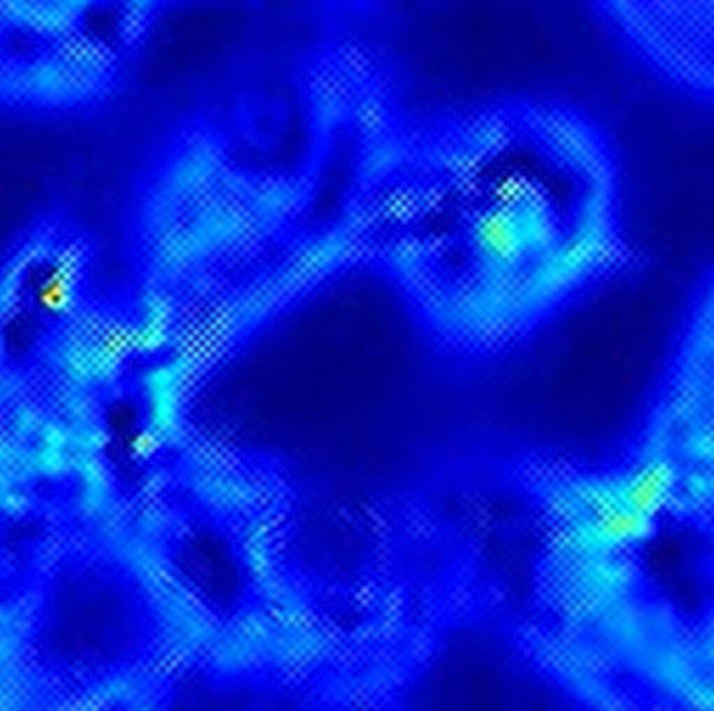
\includegraphics[width=0.8\textwidth]{figures/emergent_structures.jpg}
    \caption{A rendered frame capturing the maximally compressible path through configurations of increasing informational entropy.}
    \label{fig:emergent-structures}
\end{figure}

These findings strongly indicate that the wave-like nature of our microscopic world is not an inexplicable, quirky preference of physics.
It is the definitive algorithmic signature of a highly optimized data-compression scheme.

\section{Conclusions}

By replacing the uncomputable, discrete Kolmogorov metrics of standard AIT with a continuous, computable framework of Spectral Complexity, we establish an explicit mathematical bridge between physical structures and informational descriptions.
Solomonoff-like induction explains why we inhabit a predictable, smooth universe governed by strict symmetries rather than existing as fleeting, chaotic fluctuations: order simply compresses
better than chaos.

The wavefunction is not a mysterious physical entity; it is the universal compression algorithm of reality.

\begin{principle}{The Wavefunction Compression Principle (WCP)}
{wavefunction-as-compression}
The cosmos waves because we are observing compressed structure.

The quantum wavefunction is the universe's data-compression scheme.
\end{principle}

\section{Proof-of-Concept Videos}

\begin{itemize}
    \item \href{https://youtube.com/shorts/sfwz_O_soS4?feature=share}{Simulation History 1: Unfolding Smoothness}
    \item \href{https://youtube.com/shorts/5XYXhmOgiW8}{Simulation History 2: Emergent Geometric Symmetries}
    \item \href{https://youtube.com/shorts/XAMWDg5zX6I}{Simulation History 3: The Connected Lattice Network}
\end{itemize}
